% Working research draft; author identity and submission positioning remain open.
\ifdefined\SingleColumn
\documentclass[10pt,journal,onecolumn,draftclsnofoot]{IEEEtran}
\else
\documentclass[10pt,journal,letterpaper]{IEEEtran}
\fi
\usepackage{amsmath,amssymb,bm,graphicx,booktabs,balance}
\usepackage[hidelinks]{hyperref}
\newcommand{\Fa}{\mathbf F_a}
\newcommand{\Fd}{\mathbf F_d}
\newcommand{\pp}{\mathbf p}
\newcommand{\xx}{\mathbf x}
\newcommand{\vv}{\mathbf v}
\newcommand{\ww}{\mathbf w}
\newcommand{\at}{{\mathbf a_t}}
\newcommand{\ar}{{\mathbf a_r}}
\newcommand{\hh}{\mathbf h}
\newcommand{\ddelta}{\bm\delta}
\newcommand{\norm}[1]{\left\|#1\right\|}
\newtheorem{proposition}{Proposition}
\title{Geometry-Aware Robust Hybrid Beamforming for ISAC with Fluid Transmit Antennas}
\author{Author names and affiliations to be supplied%
\thanks{Working draft, October 2026. Numerical results are from an independent implementation; this manuscript has not been submitted.}}
\begin{document}
\maketitle
\begin{abstract}
We study single-user, single-target integrated sensing and communication with fluid transmit antennas and a fixed receive array. A geometry-aware projected descent--ascent method jointly updates hybrid beamformers and ordered antenna positions under bounded channel and steering errors. An exact spacing projection preserves geometric feasibility. Across 100 paired scenarios per regime, independently attacked weighted utility improves by 11.8\% without clutter and 10.6\% with clutter relative to retuned fixed arrays at matched gradient-call budgets. An aligned line-of-sight control has no intrinsic geometry gain. Learned position-step schedules provide no useful advantage over an equally trained scalar in this pilot.
\end{abstract}
\begin{IEEEkeywords}
Integrated sensing and communication, fluid antennas, hybrid beamforming, robust optimization, antenna positioning.
\end{IEEEkeywords}

\section{Introduction}
Fluid antennas provide spatial degrees of freedom for integrated sensing and communication (ISAC). Joint beamforming and antenna-location optimization has been studied with communication-rate and sensing-beampattern objectives \cite{zhou2024}; imperfect-CSI designs also exist \cite{hao2024}. Recent work explicitly accounts for antenna-position errors \cite{zhang2026}. Consequently, a geometry extension must distinguish its objective, hardware constraints, and evaluation from existing fluid-antenna ISAC formulations.

Wang \emph{et al.}~\cite{wang2026} consider a weighted robust communication/sensing objective with hybrid beamforming and channel/steering uncertainty. We specialize that structure to one user and one target and introduce adjustable transmit coordinates with a spatially consistent communication channel. The receive array remains fixed. Our focus is the conditional benefit of geometry under the inherited metrics and continuous-phase hybrid constraints.

We develop a geometry-aware projected gradient descent--ascent (PGDA) procedure using an exact ordered-spacing projection. A closed-form aligned line-of-sight (LOS) control identifies a regime where position changes cannot improve the optimal robust objective. Paired multipath experiments compare fluid designs with retuned uniform and fixed nonuniform arrays under common uncertainty sets and independent attacks. A position-step learning ablation tests whether a small learned schedule adds value. The study establishes empirical gains for the tested spatial distributions; it does not establish global robustness, hardware latency, or a general advantage of learned optimization.

\section{System Model and Robust Design}
\subsection{Geometry and spatial channels}
A narrowband far-field base station has $N_t$ adjustable transmit antennas, $L$ RF chains, and $N_r$ fixed receive antennas. There is one fixed single-antenna user, one target, and $J$ clutter sources. Positions are selected before a block and held fixed within it. For wavelength $\lambda$ and $k_0=2\pi/\lambda$, define
\begin{align}
 \mathcal P=\{\pp:\;&0\le p_1,\ p_{n+1}-p_n\ge d_{\min},\nonumber\\
 &n=1,\ldots,N_t-1,\ p_{N_t}\le A\},\label{eq:P}\\
 \widehat\at(\theta;\pp)&=[e^{-jk_0p_n\sin\theta}]_{n=1}^{N_t}.\label{eq:at}
\end{align}
The set is nonempty iff $A\ge(N_t-1)d_{\min}$. The receive response is $\widehat\ar(\theta)=[e^{-jk_0(n-1)d_r\sin\theta}]_{n=1}^{N_r}$.
The nominal user channel is
\begin{equation}
 \widehat\hh^H(\pp)=\sum_{k=1}^{K_c}\beta_k\widehat\at^T(\vartheta_k;\pp),
 \qquad \hh=\widehat\hh+\ddelta_h.\label{eq:h}
\end{equation}
Path gains and angles are fixed while positions are optimized. An unrelated independent channel draw after movement would not describe spatial reconfiguration. This field-response construction also changes the channel-generation law relative to the position-independent model in \cite{wang2026}. All comparisons here use the same spatial law.

Let $l=0$ denote the target and $l=1,\ldots,J$ the clutter. With fixed complex reflection coefficients $\alpha_l$, write
\begin{align}
 \mathbf H_l(\pp)&=\alpha_l\ar_l\at_l^T(\pp),\label{eq:H}\\
 \at_l&=\widehat\at(\theta_l;\pp)+\ddelta_{t,l},\quad
 \ar_l=\widehat\ar(\theta_l)+\ddelta_{r,l}.\nonumber
\end{align}
The transpose follows \cite{wang2026}. Accurate positioning, known nominal field parameters, and negligible coupling are assumed; the response errors below are not a physical position-error model.

\subsection{Signals, interference, and uncertainty}
Let $\Fd=[\mathbf f_c,\mathbf f_s]$ and $\vv_i=\Fa\mathbf f_i$ for $i\in\{c,s\}$. Independent unit-power communication and dedicated sensing symbols yield transmit signal $\vv_cz_c+\vv_sz_s$ and covariance $\mathbf R_x=\vv_c\vv_c^H+\vv_s\vv_s^H$. The user treats the sensing stream as interference, giving
\begin{equation}
 \gamma_c=\log\left(1+\frac{|\hh^H\vv_c|^2}{|\hh^H\vv_s|^2+\sigma_c^2}\right).\label{eq:gc}
\end{equation}
There is no inter-user interference or successive interference cancellation. A unit-norm filter $\ww$ extracts the target echo. Define $\mathbf q_l=\ww^H\mathbf H_l\Fa\Fd$. We retain the reference sensing metric
\begin{equation}
 \gamma_s=\log\left(1+\frac{\norm{\mathbf q_0}_2^2}{\sum_{j=1}^J\norm{\mathbf q_j}_2^2+\sigma_r^2\norm{\ww}_2^2}\right).\label{eq:gs}
\end{equation}
Both streams illuminate the target. The sum of clutter powers assumes negligible effective echo cross-correlations; independent transmit symbols alone do not remove coherent echo cross terms. Equation~\eqref{eq:gs} is an inherited MI-based surrogate, not measured detection or estimation accuracy. Natural logarithms are used; $\gamma_c$ is in nats/s/Hz.

Errors satisfy independent balls
\begin{equation}
 \norm{\ddelta_h}_2\le\epsilon_h\sqrt{N_t},\quad
 \norm{\ddelta_{t,l}}_2\le\epsilon_t\sqrt{N_t},\quad
 \norm{\ddelta_{r,l}}_2\le\epsilon_r\sqrt{N_r}.\label{eq:balls}
\end{equation}
Their product sets are $\mathcal A_h,\mathcal A_t,\mathcal A_r$. Radii remain identical across geometries and need not represent one common angle error. For $0<\rho<1$, optimize
\begin{equation}
\begin{aligned}
 \max_{\pp,\Fa,\Fd,\ww}\quad &\rho\min_{\mathcal A_h}\gamma_c+
 (1-\rho)\min_{\mathcal A_t\times\mathcal A_r}\gamma_s\triangleq U_{\rm rob}\\
 \text{s.t.}\quad &\pp\in\mathcal P,\quad |[\Fa]_{n\ell}|=1,\\
 &\norm{\Fa\Fd}_F^2=P,\quad \norm{\ww}_2^2=1.
\end{aligned}\label{eq:opt}
\end{equation}
The separate minima follow the disjoint communication and sensing errors. The weighted objective expresses a selected tradeoff and does not guarantee a minimum service level for either task.

\section{Geometry-Aware Projected Updates}
\subsection{Alternating adversary, beamforming, and positions}
Write $b=(\Fa,\Fd,\ww)$, $e=(\ddelta_h,\bm\Delta_t,\bm\Delta_r)$, and $u=\rho\gamma_c+(1-\rho)\gamma_s$. Each iteration first takes projected descent steps in the error blocks, followed by projected ascent in the three beamforming blocks using the independently implemented PGDA structure of \cite{wang2026}. Inner communication and sensing gradients use their respective component utilities; outer gradients use $u$. Momentum is $0.01$ for these inherited blocks. Gradients within each stage are evaluated simultaneously. Analog entries are mapped to their phases, $\Fd$ is rescaled after that mapping to enforce $\norm{\Fa\Fd}_F^2=P$, and $\ww$ is normalized. Each error is projected onto its ball.

The additional position step uses $\xx=\pp/\lambda$, $a=A/\lambda$, and $d=d_{\min}/\lambda$, with $b,e$ fixed at their current iterates:
\begin{equation}
 \xx^+=\Pi_{\mathcal X}(\xx+\tau\nabla_{\xx}u),\qquad
 \mathcal X=\{\xx:\lambda\xx\in\mathcal P\}.\label{eq:update}
\end{equation}
Only nominal spatial responses are differentiated. In particular,
\begin{equation}
 \frac{\partial[\widehat\at(\theta;\xx)]_n}{\partial x_n}
 =-j2\pi\sin\theta[\widehat\at(\theta;\xx)]_n.\label{eq:der}
\end{equation}
With Wirtinger derivatives $g_h=\partial\gamma_c/\partial\hh^*$ and $g_{t,l}=\partial\gamma_s/\partial\at_l^*$, the real-coordinate chain rule is
\begin{equation}
 [\nabla_{\xx}u]_n=2\Re\left\{\rho g_{h,n}^*\frac{\partial\widehat h_n}{\partial x_n}
 +(1-\rho)\sum_{l=0}^Jg_{t,l,n}^*\frac{\partial\widehat a_{t,l,n}}{\partial x_n}\right\}.\label{eq:chain}
\end{equation}
Writing any component metric as $\log(1+N/D)$ gives derivative $(DN'-ND')/[D(D+N)]$, consistent with the supplied signal model. An approximately minimized error in \eqref{eq:chain} gives a search direction, not the exact gradient of a globally minimized objective.

Classical position updates have zero momentum and try $\tau,\tau/2,\ldots,\tau/32$. The first candidate satisfying
\begin{equation}
 u(\xx^+;b,e)\ge u(\xx;b,e)+10^{-4}\nabla u^T(\xx^+-\xx)\label{eq:armijo}
\end{equation}
is accepted, up to floating-point tolerance; otherwise positions are retained. Channels are rebuilt after movement without redrawing paths. This safeguard improves the fixed-error surrogate only. Nonconvex beamforming, inexact adversaries, and momentum preclude a claim of monotone robust improvement or global convergence.

\subsection{Exact spacing projection}
For a trial vector $\mathbf y$, set $r_n=y_n-(n-1)d$ and $B=a-(N_t-1)d$. Then
\begin{equation}
 \underset{0\le z_1\le\cdots\le z_{N_t}\le B}{\arg\min}
 \sum_n(z_n-r_n)^2,\qquad
 [\Pi_{\mathcal X}(\mathbf y)]_n=z_n+(n-1)d.\label{eq:pav}
\end{equation}
An offset preserves Euclidean distances and converts spacing constraints into monotonicity. Pool-adjacent-violators (PAV) isotonic regression followed by clipping pooled values to $[0,B]$ gives the exact projection in $O(N_t)$ time. This is a standard projection construction; no general novelty of PAV is asserted. The exact active-face Jacobian averages gradients within free pooled blocks and is zero on bound-clamped blocks, except at nondifferentiable transitions. It supports the learning ablation without a straight-through approximation.

A fixed-array iteration uses two calls to the full analytic helper, each computing all six error/beamforming gradients. A fluid iteration uses a third call for \eqref{eq:chain}. Thus $G$ full calls permit $G/2$ fixed or $G/3$ fluid iterations. Equal calls do not imply equal operations: spatial reconstruction, PAV, and backtracking add work. Wall time is reported separately.

\subsection{An aligned-LOS control}
\begin{proposition}\label{prop:los}
Suppose $K_c=1$, $|\beta_1|=1$, $\vartheta_1=\theta_0$, $J=0$, $L\ge2$, and $0\le\epsilon_h,\epsilon_t,\epsilon_r<1$. Under \eqref{eq:balls}, the optimal value of \eqref{eq:opt} is independent of feasible positions and equals
\begin{align}
 U_{\rm LOS}={}&\rho\log\left(1+\frac{PN_t(1-\epsilon_h)^2}{\sigma_c^2}\right)\nonumber\\
 &+(1-\rho)\log\bigl(1+S_s(1-\epsilon_t)^2(1-\epsilon_r)^2\bigr),\label{eq:los}
\end{align}
where $S_s=|\alpha_0|^2PN_tN_r/\sigma_r^2$.
\end{proposition}
\emph{Proof:} Set $\vv_s=0$, $\vv_c=\sqrt{P/N_t}\widehat\at^*(\theta_0;\pp)$, and $\ww=\widehat\ar(\theta_0)/\sqrt{N_r}$. One unit-modulus analog column realizes $\vv_c$; unused columns have zero digital weights. Cauchy--Schwarz and the reverse triangle inequality give the ball minima in \eqref{eq:los}. Conversely, feasible errors $\ddelta_h=-\epsilon_h\widehat\hh$, $\ddelta_{t,0}=-\epsilon_t\widehat\at$, and $\ddelta_{r,0}=-\epsilon_r\widehat\ar$ bound every feasible design above by the same component values, using total power $P$ and unit receive norm. Both bounds are attained by the stated design. $\square$

A finite solver can leave this optimum. Improvement over a degraded fixed-array iterate is therefore insufficient evidence of intrinsic geometry gain.

\section{Numerical Evaluation}
\subsection{Paired scenarios and evaluation protocol}
We use $N_t=N_r=8$, $L=4$, $d_r=\lambda/2$, $A=3.5\lambda$, $d_{\min}=0.25\lambda$, $\rho=0.8$, $\sigma_c^2=\sigma_r^2=1$, $P=10^{5/10}$, and all $\epsilon=0.05$. Wavelength $0.01$ m only converts units. All methods have the same aperture, power, antenna count, RF chains, and error sets. A half-wavelength uniform linear array (ULA) and one nonuniform random array fixed across all splits/scenarios are controls. Fluid designs start from the ULA. Beamforming initialization uses nominal channel phases and target matching, with communication/sensing power split 90/10 in multipath and 100/0 in LOS.

Three regimes each have disjoint 64/32/100 training/validation/test scenarios. A is aligned LOS, with target angle uniform on $[-50^\circ,50^\circ]$ and unit-magnitude random-phase user gain. B/C use four independent complex Gaussian path gains with normalized variances proportional to $(0.75^2,0.4^2,0.4^2,0.4^2)$. The dominant departure angle is uniform on $[-30^\circ,-20^\circ]$, and other angles on $[-65^\circ,65^\circ]$. The target is uniform on $[25^\circ,35^\circ]$ in B and $[20^\circ,30^\circ]$ in C. B has no clutter; C has one clutter source $8^\circ$--$12^\circ$ beyond the target. Reflection gains are zero-mean complex Gaussian with variances $10^{2/10}$ for the target and $10^{3/10}$ for clutter. Gains remain fixed during each solve.

Inner/outer steps use the validation grid $\{0.01,0.05,0.2\}\times\{0.001,0.005,0.02\}$. Long ULA and fixed-random runs are retuned at their budgets. Fluid uses ULA beamforming steps and selects a position step from $\{0.005,0.02,0.08\}$. Test performance does not select these settings.

Evaluation freezes positions and beamformers. Communication and sensing errors are searched separately over \eqref{eq:balls}. Candidates include zero errors, terminal optimizer errors, and five random feasible starts; independent searches use 50 projected-Adam steps and nested 50/200/1000-step projected-gradient budgets. Best-so-far retention and a shared union of candidates from compared designs are used, with each candidate evaluated at the recipient's frozen geometry. Utility is the weighted sum of lowest component utilities found. It is an \emph{upper bound} on the unknown exact robust utility, not a global certificate. A additionally uses exact feasible adverse-error candidates.

\begin{table}[t]
\caption{Attacked utility at 360 full gradient calls; 100 paired scenarios. Interval is for fluid minus ULA.}
\label{tab:main}\centering\footnotesize\setlength{\tabcolsep}{3pt}
\begin{tabular}{ccccc}\toprule
Case & ULA & Fixed random & Fluid & Paired 95\% interval\\\midrule
A & 3.5278 & 3.5132 & 3.5226 & [-0.0057, -0.0046] \\
B & 2.9688 & 3.0021 & 3.3186 & [0.3299, 0.3703] \\
C & 2.6602 & 2.6804 & 2.9409 & [0.2557, 0.3051] \\
\bottomrule

\end{tabular}
\par\smallskip\scriptsize A uses the analytic ULA optimum instead of a degraded finite solver. B/C use 180 fixed or 120 fluid iterations.
\end{table}
\begin{figure}[t]\centering
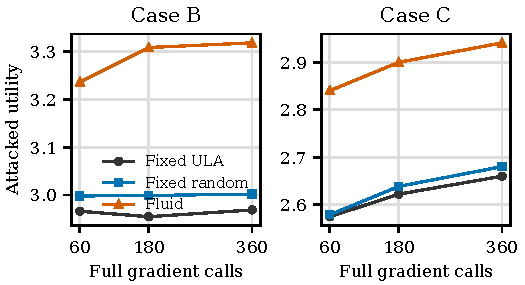
\includegraphics[width=\columnwidth]{figures/budgets.pdf}
\caption{Independent attack evaluation versus design gradient budget. ULA uses validation-retuned long runs; all curves average the same 100 scenarios per case.}\label{fig:budget}
\end{figure}

\subsection{Geometry gains and the communication--sensing balance}
Table~\ref{tab:main} shows fluid gains of 0.3498 (11.8\%) in B and 0.2807 (10.6\%) in C over retuned ULA. Paired 95\% bootstrap intervals exclude zero for both tested distributions. Fixed nonuniform geometry improves modestly, but adaptive geometry achieves higher attacked utility. These comparisons condition on the initializations, spatial laws, and attack protocol. They do not prove dominance over globally optimized fixed arrays.

A instead gives $3.5226$ for fluid versus the analytic fixed-ULA value $3.5278$, consistent with Proposition~\ref{prop:los}: geometry offers no intrinsic gain, and finite updates lose some optimality. Figure~\ref{fig:budget} also shows that more iterations need not improve every nonconvex solve.

\begin{table}[t]
\caption{Component utilities at 60 full calls and warm CPU design time (median/p95 in ms).}
\label{tab:short}\centering\footnotesize\setlength{\tabcolsep}{3.2pt}
\begin{tabular}{ccccc}\toprule
Case/method & $\gamma_c$ & $\gamma_s$ & Utility & Time\\\midrule
B/ULA & 2.8290 & 3.5151 & 2.9662 & 35.9/37.3 \\
B/Fluid & 3.1185 & 3.7087 & 3.2366 & 53.0/59.4 \\
C/ULA & 2.5914 & 2.5089 & 2.5749 & 40.8/48.9 \\
C/Fluid & 2.8643 & 2.7434 & 2.8402 & 47.2/49.9 \\
\bottomrule

\end{tabular}
\end{table}
Table~\ref{tab:short} exposes both components. Fluid improves both at $\rho=0.8$ in B/C. We also retune at $\rho\in\{0.2,0.5,0.8\}$ on the same test scenarios and 60 full calls (Fig.~\ref{fig:tradeoff}). These are observed tradeoff points, not a certified Pareto frontier. In C at $\rho=0.2$, fluid increases sensing from $3.8454$ to $4.0783$ while communication decreases from $1.8694$ to $1.8265$. Weighted improvement need not improve both components or ensure user QoS.

\begin{figure}[t]\centering
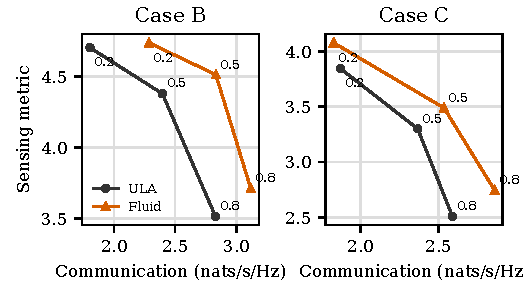
\includegraphics[width=\columnwidth]{figures/tradeoff.pdf}
\caption{Communication/sensing tradeoff at 60 full gradient calls. Labels indicate $\rho$; each point is separately validation tuned.}\label{fig:tradeoff}
\end{figure}

\subsection{Runtime, feasibility, and a learning ablation}
Timing uses one AMD EPYC 9V74 CPU thread, complex64, batch one, three warmups, and 15 paired test scenarios. Table~\ref{tab:short} includes channel reconstruction, projection, and backtracking; initialization, independent attacks, CSI acquisition, RF programming, and antenna movement are excluded. Extra overhead prevents inferring acceleration from gradient counts alone. Validation-time-selected ULA runs near fluid-20 runtime use 45 iterations in B/C: utilities are $2.9700$ and $2.5965$, with medians $63.4$ and $55.9$ ms. These are approximate runtime comparisons, not equal deadlines or hardware latency guarantees. Attack cost is recorded separately in the artifact.

All observed geometry, uncertainty, power, phase, and receive-norm residuals are below $1.5\times10^{-6}$ at a $10^{-5}$ acceptance tolerance. Independent NumPy checks and final-source replay validate saved designs. Tests cover signal conventions, spatial derivatives, exact projection, unrolled differentiation, and feasibility. Constraint feasibility follows the projections; the global robust minimum remains uncertified.

\begin{table}[t]
\caption{Position-only learning at 20 iterations/60 full calls. Means across three paired training seeds.}
\label{tab:learn}\centering\footnotesize
\begin{tabular}{cccc}\toprule
Case & Tuned plain step & Learned scalar & Learned schedule\\\midrule
A & 3.527481 & 3.527486 & 3.527486 \\
B & 3.236578 & 3.241049 & 3.241042 \\
C & 2.830243 & 2.829061 & 2.828979 \\
\bottomrule

\end{tabular}
\end{table}
Either one positive position step or 20 layer-specific steps are trained separately per regime; no compatible old spatial checkpoint is assumed. Beamforming/adversary update coefficients remain frozen although their physical iterates evolve. Both variants use the same tuned no-backtracking initialization, four Adam epochs, batch 32, learning rate $0.002$, eight updates, and three paired seeds. Full unroll differentiation includes the PAV Jacobian; a terminal 10-step training attacker is detached. Independent validation may retain epoch zero.

Table~\ref{tab:learn} shows no useful schedule advantage. B's small gain over a coarse fixed-step grid is reproduced by a learned scalar. C includes selections at initialization and trained runs that lose test utility. This neither demonstrates learned acceleration nor rules out other architectures. The 100 scenarios remain the sampling units; three fitted models are not 300 independent channels.

\ifdefined\SingleColumn\else\balance\fi
\section{Conclusion}
Within a fixed-aperture spatial model, exact spacing-projected position updates improve independently attacked hybrid ISAC utility in the tested multipath regimes. Aligned LOS has no intrinsic geometry benefit, and a small learned schedule is unnecessary in the pilot. Broader channel/aperture studies, stronger fixed-array optimization baselines, and position-error/coupling/movement models remain necessary to establish generality and practical benefit.

\noindent\emph{Reproducibility:} Configurations, raw paired outputs, and validation evidence are available at \url{https://github.com/muneefo/L2O_ISAC}, under \path{experiments/fluid_tx_single_user/}.

\begin{thebibliography}{4}
\bibitem{zhou2024} L. Zhou, J. Yao, M. Jin, T. Wu, and K.-K. Wong, ``Fluid antenna-assisted ISAC systems,'' \emph{IEEE Wireless Commun. Lett.}, vol. 13, no. 12, pp. 3533--3537, 2024, doi: 10.1109/LWC.2024.3476148.
\bibitem{hao2024} T. Hao \emph{et al.}, ``Fluid-antenna enhanced ISAC: Joint antenna positioning and dual-functional beamforming design under perfect and imperfect CSI,'' arXiv:2407.18988, 2024. [Online]. Available: \url{https://arxiv.org/abs/2407.18988}
\bibitem{zhang2026} Z. Zhang \emph{et al.}, ``Robust beamforming and antenna position optimization for MA-assisted ISAC with imperfectly positioned MAs,'' arXiv:2609.23323, 2026.
\bibitem{wang2026} L. Wang, S. A. Vorobyov, and E. Ollila, ``L2O robust hybrid beamforming for ISAC,'' \emph{IEEE Trans. Wireless Commun.}, vol. 25, pp. 18778--18794, 2026, doi: 10.1109/TWC.2026.3702925.
\end{thebibliography}
\end{document}
